\chapter{IMPLEMENTATION}%Titles must be capitalized.

In this chapter, I will introduce how I modified the KLEE to add an asynchronous mode to it as well as how do I wrapping the solver to use it as a standalone solver. Moreover, a new feature is added to KLEE. It is called ``otherside testcase generation``.

\section{Asynchronous Mode}
As I mentioned in Chapter 2, KLEE is a synchronous symbolic execution tool. KLEE will wait for the result from the solver even though it is not necessary to do so. Figure \ref{klee_control_flow} shows the control flow of KLEE. After terminating an \texttt{ExecutionState}, KLEE will ask solver to solve the constraints in that \texttt{ExecutionState} and wait for the result. Then checking if there is any \texttt{ExecutionState} waiting to be executed in the pool. However, KLEE will not use the result that it waits for. Previous research has pointed out that symbolic execution engine spends 90\% of their time in solver constraints \cite{Rakadjiev:2015:PSS:2847598.2847727}. Therefore, waiting for a result that it will not use anymore is wasting time. Alternatively, the solver can solve the constraints alone. KLEE is not helping the solver while it is waiting for the result. KLEE should keep executing other \texttt{ExecutionState} left in the pool. This improvement can significantly shorten the time for analyzing a program. In other words, the analysis task will finish much earlier than before. And the analyzing time relies on the engine's performance instead of solver's performance. 

\begin{figure}%This [h] tells LaTeX to try to put the picture here.
                 %Without it, it will go to the top of the next page.
\begin{center}
{\mbox{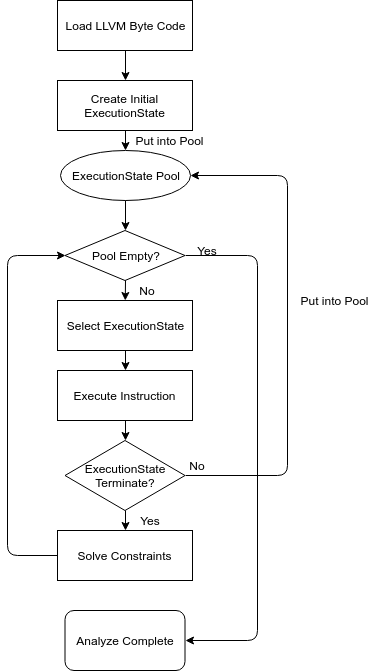
\includegraphics[height=500pt]{figures/klee_control_flow.png}}}
\end{center}
\caption{\label{klee_control_flow}KLEE Original Control Flow}
\end{figure}


To transmit queries, I decided to send out the constraints in the KQuery format using HTTP \texttt{POST} method. The decision is under following consideration. KLEE has its special data structure to represent constraints. If a query needs to be sent out, it requires data serialization. Once the solver receives the query and deserializes it, it turns out to be KLEE's data structure. Under this setting, solver becomes ``KLEE-ONLY'' because the solver does not know about other engine's data structure and unable to handle those queries from other symbolic execution engines. Also, sending queries in KQuery format reduce the work for changing backend solver. All constraints solver has their own interface. Connecting symbolic execution engine's  data structure to different solver's interface requires a solid understanding of data structure from the engine. However, if the solver only receives queries written in KQuery format, we just need to know how to connect KQuery to solver's interface if we need to replace the backend solver, even though the engine changes its own data structure in the future. Moreover, KQquery is a human readable representation. When we need to debug the solver, KQuery can make it easier. Receiving queries in KQuery has such advantages, yet nothing is perfect. Presenting constraints in KQuery needs conversion time, and the process of conversion takes longer than the serialize the data structure of the symbolic engine. At the solver side, parsing the queries in KQuery into the data structure that can be used in solver's interface also takes longer than the data deserialization. After carefully considering the trade-off between speed and scalability, I decided to transfer the query command in KQuery format instead of serializing the original data structure of the symbolic execution tool.

Once deciding how to transmit the queries to the remote solver, the rest of the implementation is straightforward. In KLEE's implementation of terminating an execution path, they first ask the solver to generate a testcase based on the constraints that the tool collected during the execution. Then delete the \texttt{ExecutionState}. In my implementation, I took out the constraints from the \texttt{ExecutionState}, then convert them into the format of KQuery and send it to the remote server via \texttt{HTTP POST} request.

% \begin{figure}[h]%This [h] tells LaTeX to try to put the picture here.
%                  %Without it, it will go to the top of the next page.
% \begin{center}
% {\mbox{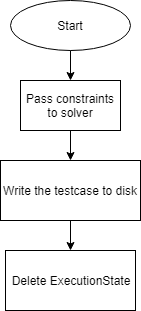
\includegraphics[height=250pt]{img/KLEE_terminate.png}}}
% \end{center}
% \caption{\label{klee_control_flow}KLEE's Workflow Terminating a State}
% \end{figure}

In addition to providing KLEE an asynchronous mode, testcases generation for a concrete input of a program is also provided. Feeding in a concrete input, if the input went through some ``forkable'' statement, then generate the testcase to hit the ``opposite'' branch. For example, Snippet \ref{get_sign} is a program get the sign of an integer, feeding a concrete input ``1'', the program will return ``positive''. In this case, the ``opposite'' branches are the return of ``negative'' and ``Zero.'' So feeding in a concrete input ``1'', the testcases generation for that concrete input will generate two testcases that contains a negative number and contains a 0 respectively in order to hit the other branch of the ``forkable'' statement. 

\begin{spacing}{1}
{
\begin{lstlisting}[frame=shadowbox, caption={Get Sign},label={get_sign}]
int get_sign(int x) {
    if (x == 0) return "Zero";
    if (x > 0) {
        return "Positive";
    }
    else {
        return "Negative";
    }
}
\end{lstlisting}
}
\end{spacing}

However, during the implementation, there is a problem need to be addressed, that is, once the input is concrete, KLEE will determine that there is no ``forkable" in the target binary. Figure \ref{br_syntax} indicate the syntax of LLVM \texttt{br} instruction. When a \texttt{br} instruction was hit, KLEE will check the \texttt{cond} of this instruction. The result is one the following, \texttt{True}, \texttt{False}, \texttt{Unknown}. \texttt{True} means the \texttt{cond} in this instruction is always true, for example, \texttt{if (1 == 1)}. \texttt{False} means the \texttt{cond} always be false, for example, \texttt{if (1 == 2)}. \texttt{Unknown} means the \texttt{cond} is can either be true or false. This situation happens only when there is a symbol involved in the \texttt{cond}. The term ``forkable" means the component of an instruction is not concrete or there are two destinations for this instruction. \texttt{br}, \texttt{switch}, \texttt{alloc} and \texttt{load} are some potential forkable instructions.

\begin{figure}[h]%This [h] tells LaTeX to try to put the picture here.
                 %Without it, it will go to the top of the next page.
\begin{center}
{\mbox{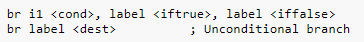
\includegraphics[height=40pt]{figures/LLVM_br_instruction_syntax.png}}}
\end{center}
\caption{\label{br_syntax}LLVM Br Instruction Syntax}
\end{figure}

Without knowing which line of instructions is forkable, generating testcases for the opposite branch is impossible. Potential forkable instructions can appear many times in a normal program, but only a few of these instructions are involved with the target symbol. If the instruction is not ``forkable,'' we have no idea if the instruction is involved with the symbol. More importantly, if an instruction cannot be forked, there is no opposite branch of that instruction. To solve this issue, I decided to use path log to guide the symbolic execution. The target binary will be run twice. The first time, a concrete input will be fed. During the execution, all of the potential forkable instructions will be logged. In my implementation, I will log four types of instruction I mention previously. For \texttt{br} instruction, instruction id and the result of \texttt{cond} will be logged. For \texttt{switch} instruction, instruction id and index of the successor will be logged. For \texttt{alloc} instruction, instruction id and allocation size will be logged. For \texttt{load} instruction, instruction id and the offset will be logged. The second run will run the program with the symbol. While exploring the path, the path log that collected during the first time can guide the execution. All the log information will be kept in a queue. If hitting the potential forkable instructions, matched the instruction id and the \texttt{cond} result/successor id/allocation size/offset with the path log in queue. If the instruction cannot be forked, the log and the execution should be the same. If it is forkable, use the log information to replace those corresponding components in the instruction. This step ensures the execution will choose the same path as the concrete input do. In \texttt{br} instruction, what will be added to constraints is based on the log. If the log is false, the negation of \texttt{cond} will be added. Otherwise, \texttt{cond} will be added. To produce the testcase that hit the other side, all we need to do is to connect the constraints (not including the newly added one) and negation of \texttt{cond} or \texttt{cond} regarding the log with the \texttt{AND} logic operator. Then we can ask solver to solve the constraints to produce a testcase that hit the opposite side. Figure \ref{testcase_generation} describes the workflow of this feature.

\begin{figure}%This [h] tells LaTeX to try to put the picture here.
                 %Without it, it will go to the top of the next page.
\begin{center}
{\mbox{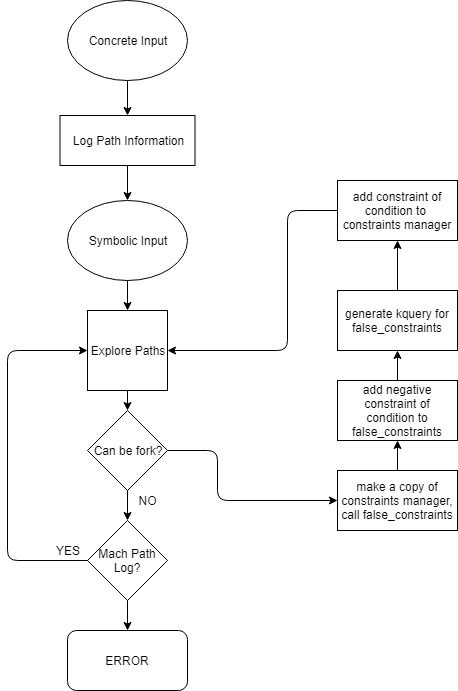
\includegraphics[height=500pt]{figures/testcase_generation.png}}}
\end{center}
\caption{\label{testcase_generation}Workflow of Generating Testcase for ``Opposite Brance''}
\end{figure}

\section{Remote Solver}

The remote solver has two part. A server that handles the HTTP request it receives and a Solver solve the queries received by a solver. Figure \ref{arch} illustrates the architecture of the remote solver. Once a \texttt{String} arrives at the Server, it will first create a file with a unique name and write the \texttt{String} it receives to the file. Then append the absolute path of that file to another file called ``Monitor'' file. This file is responsible for communicating between the server and solver. 

\begin{figure}[h]%This [h] tells LaTeX to try to put the picture here.
                 %Without it, it will go to the top of the next page.
\begin{center}
{\mbox{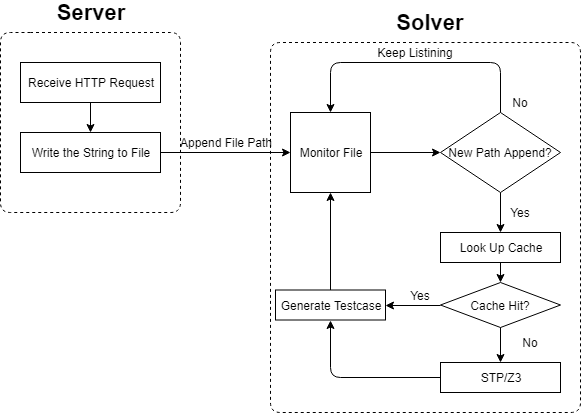
\includegraphics[height=300pt]{figures/arch.png}}}
\end{center}
\caption{\label{arch}Remote Solver Architecture}
\end{figure}

The solver is listening to ``Monitor'' file using \texttt{inotify}, which is a Linux kernel subsystem that acts to extend filesystems to notice changes to the filesystem and report those changes to applications \cite{inotify}. There are two threads in the solver. The first one is the watching module, responsible for retrieving the new appended file and push it into a thread-safe queue waiting to be solved. The other thread is the solver itself. If the queue is not empty, poping a file path once a time. Then read the content of that file, parse the content. Thanks to KLEE's implementation, they have a parse that can parse a \texttt{String} in the format of KQuery and can be used in the STP/Z3 solver directly. After parsing, the solver will check the cache map to see if there is any hit. If so, get the result from the cache map and save it as testcase. Otherwise, pass it to the solver and insert the \texttt{<constraints, result>} pair to the cache map for future use. Also, this solver will support the constraints independence optimization. 

\section{``Otherside'' Testcase Generation}
As we all know, symbolic execution is used to discover all the feasible paths of a binary, however, in some situation, we do not need to know all the paths but just some paths. To address this problem, I added a new feature to KLEE and it is called ``Otherside'' testcase generation. 

The term ``otherside" is refer to control flow direction. In the programming language level, a \texttt{if} statement may have many branches. However, in assembly level, all the ``if" statements have just two branches -- either ``True" or ``False". So, if a \texttt{br} instruction is ``True", its otherside is ``False". Otherside testcase generation aims to generate testcases that covered the otherside of the branches for a given input. Code snippet \ref{odd_or_even} shows a program that determine a number is a even number. For the given input ``2", the otherside testcase generation will generate a testcase ``1" since the this testcase will cover the otherside of the ``if" branch of the program.

\begin{spacing}{1}
{
\begin{lstlisting}[frame=shadowbox, caption={Is Even},label={odd_or_even}]
bool isEven(int n) {
    if (n % 2 == 0) {
        return True
    }
    else {
        return False
    }
}
\end{lstlisting}
}
\end{spacing}
\pagebreak
To achieve this goal, we need a concrete input for the target binary as the given input. During the execution of the given input, we need to log the path that it travels through. Then, we reset the program and make the input as symbol and use the log we collected to guide the symbolic execution.

In KLEE, instructions that will cause a ``fork'' action is the log we need to collected -- they are \texttt{br}, \texttt{switch} and \texttt{alloc}. And during the second run, we will use symbol as the input of the target binary. When it needs to fork, the path log that collected by the first run will be used to guide the execution. At the same time, the opposite condition will be concatenated to constraints using ``AND'' logic operator and send to the remote solver for testcase case generation purpose.

After two runs, we will have testcase that can hit all the opposite branches of the original concrete example.